\documentclass[titlepage]{article}
\usepackage[utf8]{inputenc}
\usepackage{amsthm}
\usepackage{mathtools}
\usepackage{graphicx} %obsluga grafiki
\usepackage{epstopdf} %obsluga eps
%\usepackage[nottoc, notlof, numbib]{tocbibind} % wyswietlenie bibliografii w spisie tresci
\usepackage{url}
\usepackage[justification=centering]{caption}
\usepackage{float}

\title{Research Skills and Methodologies\\Path Optimization of 3D Printer}
\author{Michał Kowalski, 195447\\Piotr Lechowicz, 195651}
\date{}

\begin{document}
\maketitle

\section{Introduction}
Nowadays 3D printing is one of the fastest developing technologies. It allows us to convert digital 3D models into solid 3 dimensional objects. It is commonly used in prototyping because it allows to make 3D object without a need to use forms. The main advantages of 3D printing technology are: low cost of the printer, low cost of printing object, variety of materials and variety of technologies.
To use this technology, we need to:
\begin{enumerate}
\item create a 3D model of our object,
\item "cut" (convert) it into set of very thin layers,
\item choose path for printing tool.
\end{enumerate}
Our path should consist of points from layer currently being printed. Tool have to visit each point exactly once and can move without printing. Task is to minimize "cost" of moving between all succeding points in our path. We can calculate it for each pair in (at least) three ways:
\begin{enumerate}
\item distance between points,
\item time needed for move from one to next,
\item energy needed for that move.
\end{enumerate}
We are assuming that our printing tool is a point moving on two perpendicular axes.

Another task was to write an environment, which will deliver layers for algorithms, provide methods commonly used in finding path, and will save and show results in human-friendly way, including graphical representation of found path. It should also be open to addition of new algorithms.

\pagebreak

\section{Mathematic description of problem}
Given:
\begin{itemize}
\item printing layer as an array (size n x m) of binary points, where
\begin{equation}
\label{layer}
X_{i,j}=\left\{ \begin{array}{rl}
 1 &\mbox{if printing point} \\
 0 &\mbox{otherwise}
       \end{array} \right. \mbox{and} i \in n, j \in m
\end{equation}
\item cost for move between two points calculated in one of three possible ways:
\begin{itemize}
\item minimum distance
\begin{equation}
\label{distance_cost}
L_{P_{a,b}, P_{c,d}} = \sqrt{(a-c)^2+(b-d)^2}
\end{equation}
\item minimum time (only axis which need to move more)
\begin{equation}
\label{time_cost}
L_{P_{a,b}, P_{c,d}} = max(|a-c|, |b-d|)
\end{equation}
\item minimum energy (sum of movements, due to separate engines)
\begin{equation}
\label{energy_cost}
L_{P_{a,b}, P_{c,d}} = |a-c|+|b-d|
\end{equation}
\end{itemize}
where $a, c \in n$ and $b, d \in m$.
\end{itemize}

Find:
\begin{itemize}
\item order of visiting points $V=[X_1, X_2, ..., X_p]$ where \textit{p} is count of points in layer,
\item total cost of path consisting of visiting points $L=\sum\limits_{k=2}^p (L_{X_{k-1}, X_k})$,
\item time of calculations for each considered algorithm,
\end{itemize}
such that length of path and time of calculations are minimized.

\pagebreak
\section{Description of Algorithms}
Following algorithm were implemented:
\begin{itemize}
\item Left-To-Right algorithm
\item Snake algorithm
\item Edge Following algorithm
\item Greedy algorithm
\item Two Opt algorithm
\item Greedy Two Opt algorithm
\item Harmony Search algorithm
\item Greedy Harmony algorithm
\item Simulated Annealing algorithm
\item Greedy Annealing algorithm
\end{itemize}

All implementations of algorithms are based on superclass, which makes all necessary communication between environment and algorithm, like:
\begin{itemize}
\item setting up an algorithm, e.g. getting a layer to print,
\item sending results of algorithm to rest of application,
\item measuring time of calculations.
\end{itemize}
Therefore algorithms only have to do all calculations in method returning a path, and optionally set up all variables in separate method. It also simplifies adding new algorithms, because all they have to do is implement this method, and they have to be added to list of algorithms.

\subsection{Left-To-Right algorithm}
This algorithm was created mostly for testing purposes. It had to be as simple as possible, and still find correct route, so it allows to test how environment works with algorithms in general.

Algorithm starts in top-left corner and goes line-by-line from left to right, adding to route all points on its way. And because only point to print are on found route, printer will go straight from last point in one line, to first in next one containing any points. Behaviour of this algorithm is similar to traditional paper printes.

\subsection{Snake algorithm}
This algorithm is an improvement of Left-To-Right algorithm. Instead of going always from left to right, it finds a closer end of next line containing points, and then goes to another end of it. Differences between them are show on figure \ref{img:ltr-vs-snake}

\begin{figure}
\begin{center}
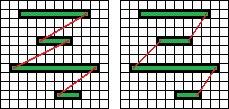
\includegraphics[scale=2]{img/ltr-vs-snake}
\caption{Left-To-Right algorithm on the left, Snake algorithm on the right}
\label{img:ltr-vs-snake}
\end{center}
\end{figure}

\subsection{Edge Following algorithm}
This algorithm starts from edge of a shape on a layer, and tries to get to the middle of it, and later choose next shape.

%------------------------------------subsection greedy-------------------------

\subsection{Greedy algorithm}

A greedy algorithm is an algorithm which always makes the choice that looks best at the moment. It makes a locally optimal choice with the hope of finding a global optimum. Greedy algorithms do not always yield optimal solution nevertheless they may give solution that approximate a global optimal solution in a reasonable time. Commonly greedy strategy for the travelling salesman problem is as follows: at each stage visit an unvisited point nearest to the current city. In case of this particular problem of path finding in 3D printer, locally optimal solution was slightly modified.

Lets consider an example where locally optimal solution is based only on distance between two points. In all examples distance between two adjacent points equals to one. Figure \ref{img:greedy/example-points-on-layer} shows example layer with few points. If optimal choice is made only by considering distance, the path would look as it is shown in the figure \ref{img:greedy/example-path-sol-1}.

\begin{figure}[H]
	\begin{center}
		\begin{minipage}{.45\linewidth}
			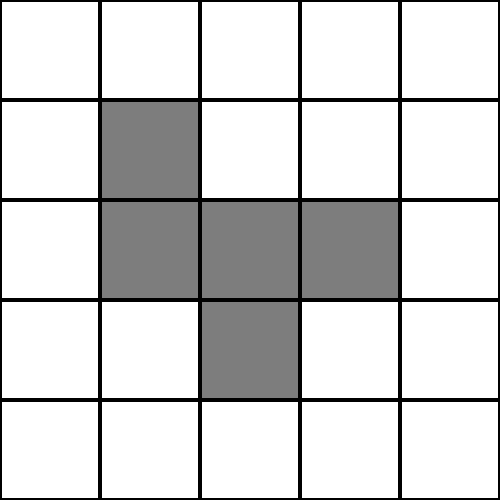
\includegraphics[width=\textwidth]{img/greedy/example-points-on-layer.png}
			\caption{Example points on layer}
			\label{img:greedy/example-points-on-layer}
		\end{minipage}
		\hspace{.05\linewidth}
		\begin{minipage}{.45\linewidth}
			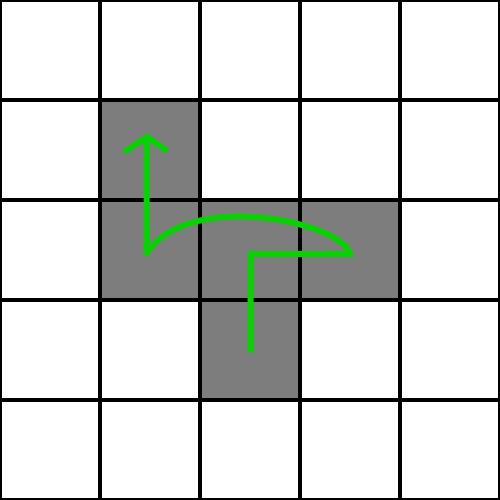
\includegraphics[width=\textwidth]{img/greedy/example-path-sol-1}
			\caption{Path number 1 for example layer}
			\label{img:greedy/example-path-sol-1}
		\end{minipage}
	\end{center}
\end{figure}

\[ L = 5 \mbox{ ,where }L \mbox{ - length of the path}\]

On the other hand if we begin to consider locally optimal solution not only based on distance between source and target points but also on number of adjacent points to target point, we can notice that in some cases it is better to choose point a little further but with lower number of adjacent points. It is illustrated in the figure \ref{img:greedy/example-path-sol-2}.

\begin{figure}[H]
	\begin{center}
		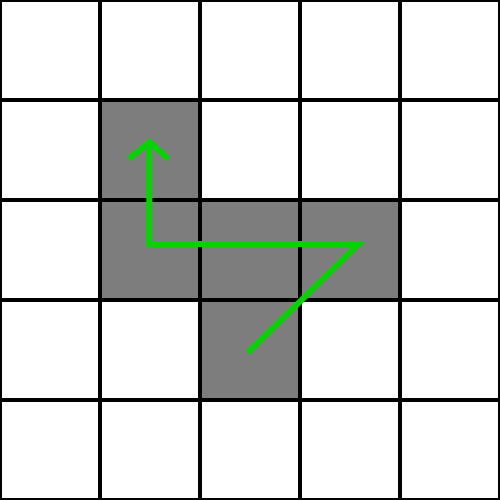
\includegraphics[width=0.5\textwidth]{img/greedy/example-path-sol-2}
		\caption{Path number 2 for example layer}
		\label{img:greedy/example-path-sol-2}
	\end{center}
\end{figure}

\subsection{Two Opt algorithm}

\subsection{Greedy Two Opt algorithm}

\subsection{Harmony Search algorithm}

\subsection{Greedy Harmony algorithm}

\subsection{Simulated Annealing algorithm}

\subsection{Greedy Annealing algorithm}

\section{Experiments}
\subsection{Environment}
\subsection{Test layers}
Images used as test layers are in "img" directory added to this report.

\section{Results}
For very short calculations, measured time can has very big differences between one measurement and another one with the same algorithm/params.

All result images and text files are added to this report in "results" directory.

\section{Conclusion}
\begin{figure}
\begin{center}
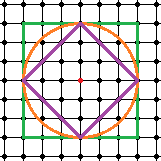
\includegraphics[scale=2]{img/costs}
\end{center}
\caption{Points with cost from red point equal to 3.\\Orange for distance, green for time, and violet for energy}
\label{cost_function_representation}
\end{figure}
As we can see on figure \ref{cost_function_representation}, when algorithm is seeking for closest point, it finds different ones, depending on cost function type. Therefore, if algorithm makes use of this, the results will vary.

Snake algorithm usually provides almost 2 times better results than Left-to-Right, in similar time. For some layers it also provides optimal (or close to it) paths, whereas for other it can give results multiple times worse than optimal.

Not only count of points, but also size of whole layer (even if points are only in the middle) can have influence on results or time of calculations, e.g. when algorithm is searching for closest point.

\section{Own contribution}
Michał's contribution:
\begin{itemize}
\item application for tests and graphical representation of results,
\item Left-To-Right algorithm,
\item Snake algorithm,
\item Edge-Following algorithm,
\item layers sp-5 and sp-6,
\item time and energy cost functions,
\item experiments and this report.
\end{itemize}
Piotr's contribution:
\begin{itemize}
\item layers from sp-7 to sp-9,
\item experiments and this report. 
\end{itemize}

\section{References}

\end{document}